\documentclass{article}
\usepackage[utf8]{inputenc}
\usepackage{graphicx}
\usepackage{amsmath}
\usepackage{float}
\usepackage{lscape}
\usepackage{subcaption} %Side by side images

%User defined commands
\newcommand*\mean[1]{\overline{#1}}

\newcommand*\hadamarddiv{\obslash} %Hadamard division

\title{Project-thesis}
\author{Erik Rundhovde M\o renskog}
\date{September 2019}

\begin{document}

\maketitle

\tableofcontents

\section{Abstract}
This thesis will describe how to detect parameters in garbage 

Waste is a huge resource that is in large degrees wasted in todays society. In Norway 39\% is recycled, 57\% is burned for energy (Waste to energy or WtE) and 2\% goes into landfills \cite{EnvironmentGlance20152015} p.50. This thesis will look into one way of analyzing waste before burning. The idea is to use a spectrometer in the visible range combined with a camera to monitor the waste as it is inserted into the waste can. This will allow us to over time find parameters describing the waste, and possibly the objects the waste consists of. 


\section{Introduction}
Hyperspectral imaging is extremely useful for classifying substances from a distance, but it is also very expensive. This paper will study if it is possible to use the much cheaper combination of camera and spectrometer instead of a hyperspectral camera in ideal situations. 
Hyperspectral imaging is a growing technology for remote sensing. The advantage is that you can get high spectral resolution in combination with high spatial resolution, usually 1 dimension for each. The proposed alternative is one where a camera is combined with a spectrometer. The camera will be able to give high spatial resolution in 2D, while the spectrometer will provide high spectral information for the same sample. The theoretical setup is shown in figure \ref{fig:measurement_setup}. 


\begin{figure}[hb]
    \centering
    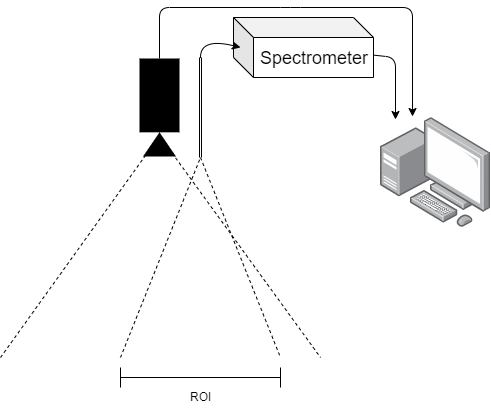
\includegraphics[width=1\textwidth]{figures/pt_setup.png}
    \caption{Measurement setup}
    \label{fig:measurement_setup}
\end{figure}


\section{Theory}
%Need theory about ccd? It is not really relevant is it?
%Need theory about the different uses of the same sensor in spectrometer and camera

\subsection{Spectrometry }
Spectrometer is a widely used tool for analyzing substances. It is a remote sensing tool that give good spectral information about all the light that enter the fiber. Because of this it can be used to give an average spectrum of the area under the acceptance cone of the fiber. 

\subsection{Reflection}
Reflection of light describes the notion of light hitting materials and getting a change of path due to the exchange of energy with the material. There are two extremes when we talked about reflection:

\textbf{Specular reflection} denotes the case where the light is reflected in unison manner from the sample, all in one direction. This concept is shown in figure \ref{fig:specular_reflection}.

\begin{figure}[h!]
    \centering
    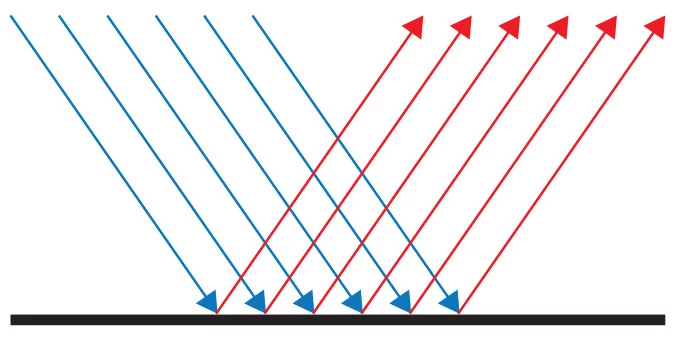
\includegraphics[width=0.5\textwidth]{figures/theory/Specular-Reflection.png}
    \caption{Example of specular reflection \cite{SpecularReflectionOcean}}
    \label{fig:specular_reflection}
\end{figure}

\textbf{Diffusive reflection} denotes the case where the light is scattered in every direction. This concept is show in figure \ref{fig:diffusive_reflection}.

\begin{figure}[h!]
    \centering
    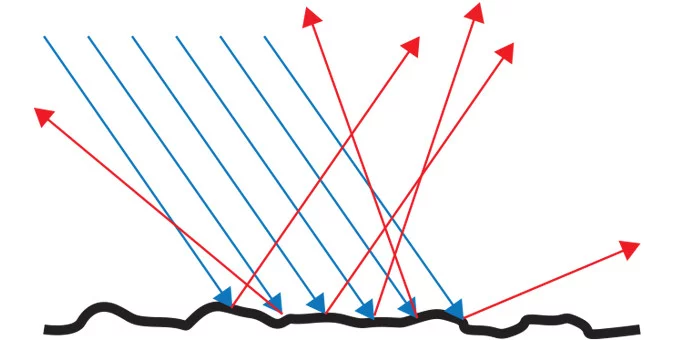
\includegraphics[width=0.5\textwidth]{figures/theory/Diffuse-Reflection.png}
    \caption{Example of diffusive reflection \cite{DiffuseReflectionOcean}}
    \label{fig:diffusive_reflection}
\end{figure}

Both of these reflection types are ideal and all real reflection will be a combination of these two. Not even the best available mirrors exhibit perfectly specular properties. It is however useful to have two extremes to compare the results too. 


%TODO: Im not sure yet about including these
%\subsubsection{Specular} 
%\subsubsection{Diffusive}
%\subsection{Relative reflection}

\section{Definitions}
This section will introduce all the math notation and equations that will be used in the paper. 

\subsection{Image}

Each pixel of the image will be described by a vector (\ref{eq:vector_pixel_bgr}), where each point on the vector describes one of the colors blue (B), green (G) and red (R).  This together gives the color combination of each pixel. Each color is an unsigned integers. 


\begin{equation}
    \label{eq:vector_pixel_bgr}
    \vec{p}_{ij} = [B,G,R]
\end{equation} 

One whole image will be stored in a matrix where each element of the matrix is a vector described by (\ref{eq:vector_pixel_bgr}). The matrix $A_{N\cdot M}$, where $N$ is the number of rows and $M$ is the number of columns, is shown in (\ref{eq:image_matrix})

\begin{equation}
    \label{eq:image_matrix}
    A = A_{N\cdot M} =  
    \begin{bmatrix}
        \vec{p}_{11} & \vec{p}_{12} & \cdots & & \vec{p}_{1M}  \\
        \vec{p}_{21} & \ddots &        &       &                \\
        \vdots       &        &\vec{p}_{ij}&   & \vdots          \\
                     &        &        & \ddots&                  \\
        \vec{p}_{N1} &        &        &       & \vec{p}_{NM}  
    \end{bmatrix}
\end{equation}

A second matrix to introduce is the special case where the image is the reference image, this special case will be denoted as $A_0$.

\subsubsection{Average}

An important equation later is the one that takes the spatial average of the matrix, this is done with (\ref{eq:spatial_sum}).
\begin{equation}
    \label{eq:spatial_sum}
    \mean{\vec{p}} = \frac{1}{NM} \sum_{i=0}^{N-1} \sum_{j=0}^{M-1} \vec{p}_{ij}
\end{equation}


\subsubsection{Hadamard division}
Element wise division will be used to compare two pictures, and is defined by the Hadamard division \cite{HadamardDivisionInfixed}:
\begin{equation}
    \label{eq:element_wise_division_image}
    A \oslash  A_0  \frac{A_{ij}}{A_{0ij} } %TODO
\end{equation}


\subsection{Spectrum}
\label{sec:spectrum}

The spectrum read from the spectrometer is saved in a $C x 2$ matrix, where $C$ is the dataset length, the first column is the wavelength ($\lambda$) and the second column is the corresponding intensity (\ref{eq:intensity})
\begin{equation}
    \label{eq:intensity}
    I = I(\lambda)    
\end{equation}

\begin{equation}
    \label{eq:intensity_0_background}
    I_0 = I_0(\lambda)
\end{equation}

We will also define a value (\ref{eq:intensity_0_background}) which is $I$ for the special case where the spectrum is muffin the background spectral response without any objects. From these definitions we define relative reflectance $RR$ (\ref{eq:relative_reflectance}). 

\begin{equation}
    \label{eq:relative_reflectance}
    RR = \frac{I}{I_0}
\end{equation}


We further introduce the notion of finding the spectrum corresponding to one color in the camera. Each pixel in the camera measures the light intensity for blue, green and red with a certain quantum efficiency given by the manufacturer. These values will be represented in a vector (\ref{eq:quantum_efficiency}) with three values corresponding to each wavelength $\lambda$. These values will represent how well each color is received by the camera and will be a float between zero and 1. 

\begin{equation}
    \label{eq:quantum_efficiency}
    \vec{QE}(\lambda)    
\end{equation}

This value can theoretically be used to relate the relative picture values with the relative reflectance values. This would be a major advantage as it can give us an insight into the noise factor affecting the sensor fusion.  
The spectral equivalent of spatial sum (\ref{eq:spatial_sum}) is to take the integral of the graph and divide it by the wavelength range (\ref{eq:average_integral}). The trapezoidal rule was used to approximate the integral \cite{TrapezoidRuleMathematical}. 

\begin{equation}
    \label{eq:average_integral}
    \mean{\vec{RR}} = \frac{1}{\lambda_1 - \lambda_0} \int_{\lambda_0}^{\lambda_1} RR \cdot \vec{QE} \,\mathrm{d}\lambda 
\end{equation}

\section{Method}
Both the spectrums and the images will be analysed using spectrometer methods, this will open up for the opportunity to pre-process spectral and spatial data in the same way. We will then hopefully be able to compare the data more directly. The spectrometer processing method we want to use is relative reflectance ($RR$). Since this method is also being used with the spectrometer, it will be denoted $RR'$ whenever it is used for imaging. As can be seen from (\ref{eq:relative_reflectance}), relative reflectance is done by dividing the interesting values with a reference. The translation to image processing must be to divide every image pixel with a pixel value from a reference image. For comparing values with the spectrometer it is fully ok to do this division as long as the reference image is non-zero for all pixels. For that reason it is important with a well lit and preferably white background. 


One problem with this method is that images can only be visualized as three sets of integers between 0 and 255, i.e. the colors blue, green and red. Therefore we divide the division into to two cases when visualizing; reference divided by image and image divided by reference. We will denote the product $RR'_{negative}$ for the reference divided by image case, and $RR'_{positive}$ for the image divided by reference case. The processing can be view in figure \ref{fig:image_visualization_program_flow} 

\begin{figure}[h]
    \centering
    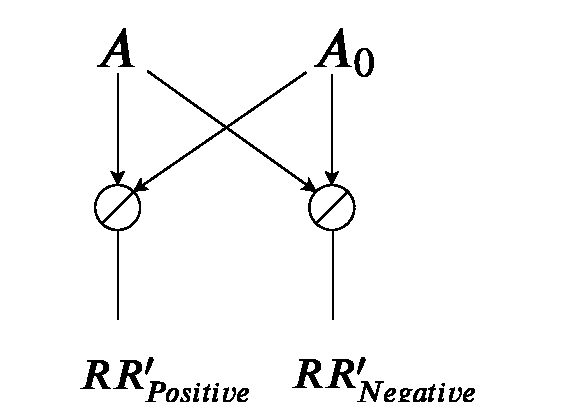
\includegraphics[width=0.5\textwidth]{figures/image_program_flow.pdf}
    \caption{Image visualization process flow}
    \label{fig:image_visualization_program_flow}
\end{figure}


\subsection{Spectrum processing}
\label{sec:spectrum_processing}

\begin{figure}[h]
    \centering
    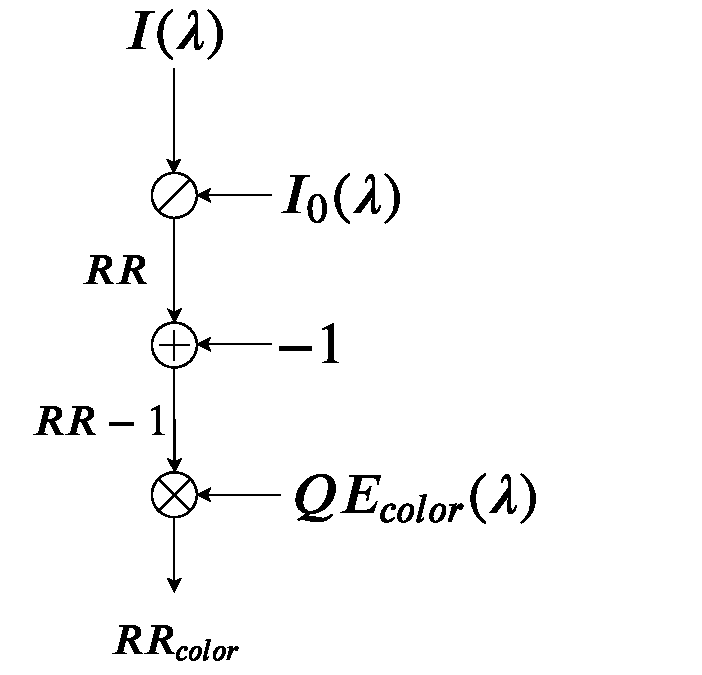
\includegraphics[width=0.5\textwidth]{figures/thesis_program_flow.pdf}
    \caption{Spectrum process flow}
    \label{fig:spectrum_process_flow}
\end{figure}

\subsection{Correlating Spectrometer to Camera}
\label{sec:method_correlating_spectrum_to_camera}
To get an idea of how well calibrated the camera is to the spectrometer and vice versa I propose the following calculation: 
Take the spatial average across the image from the camera and divide it with the spectral average of the spectrometer. 

\begin{equation}
    \label{eq:correlating_spectrum_to_camera}
    K = \frac{\mean{\vec{p}}}{\mean{RR}}
\end{equation}

This process is shown in figure \ref{fig:correlating_spectrum_and_image}.

\begin{figure}[h]
    \centering
    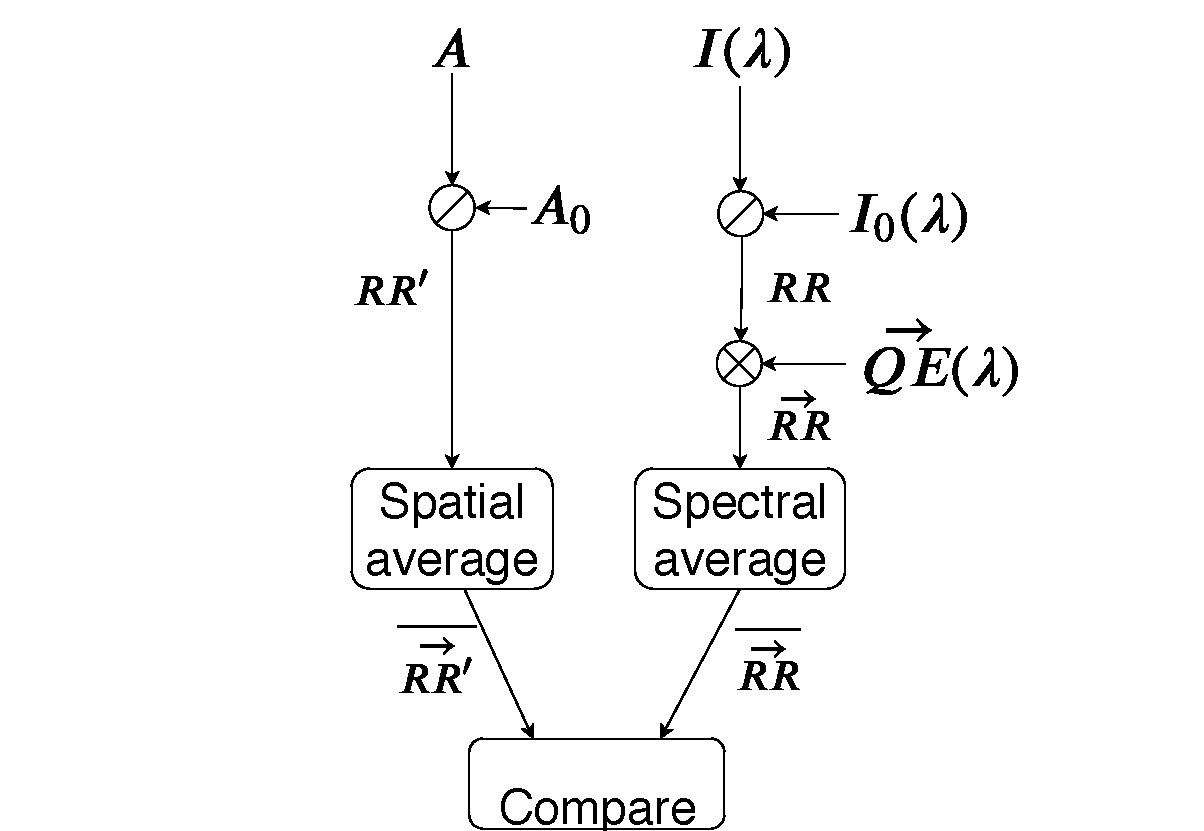
\includegraphics[width=0.5\textwidth]{figures/image_comparison_with_spectrometer.pdf}
    \caption{Correlating value between image and spectrum}
    \label{fig:correlating_spectrum_and_image}
\end{figure}


\subsection{Light}
Light is a crucial part of this project, as it is the source of input for both the camera and the spectrometer. It's also the link between the two sensors. The choosing of a sensor that can support both sensor types is therefore paramount. The camera is less selective on the spectral properties of the light source as it only requires a light source that is approximately white, i.e. have similar amounts of red, green and blue "wavelengths". It is however more selective in the spatial region as it can arise more problems for the camera if the lighting creates a lot of shadows or local problems like strong specular reflection making the pixel go into saturation. As implied the spectral properties of the light is more important for the spectrometer. For the spectrometer we want the spectrum to be as flat as possible. 

The characterization of the light source will be based on considerations from \cite{martinPracticalGuideMachine}, but also unfortunately be limited by available sources at the lab. % This paper provides a longer checklist, that can be simplified greatly under the following conditions: Stationary objects,


\section{Results}
The photos and spectrums where taken inside a lab with no external lights, and the real setup is as shown in figure \ref{fig:picture_of_setup_unlit}. %TODO: Change this figure into the side by side, lit - unlit


\begin{figure}[h]
    \centering
    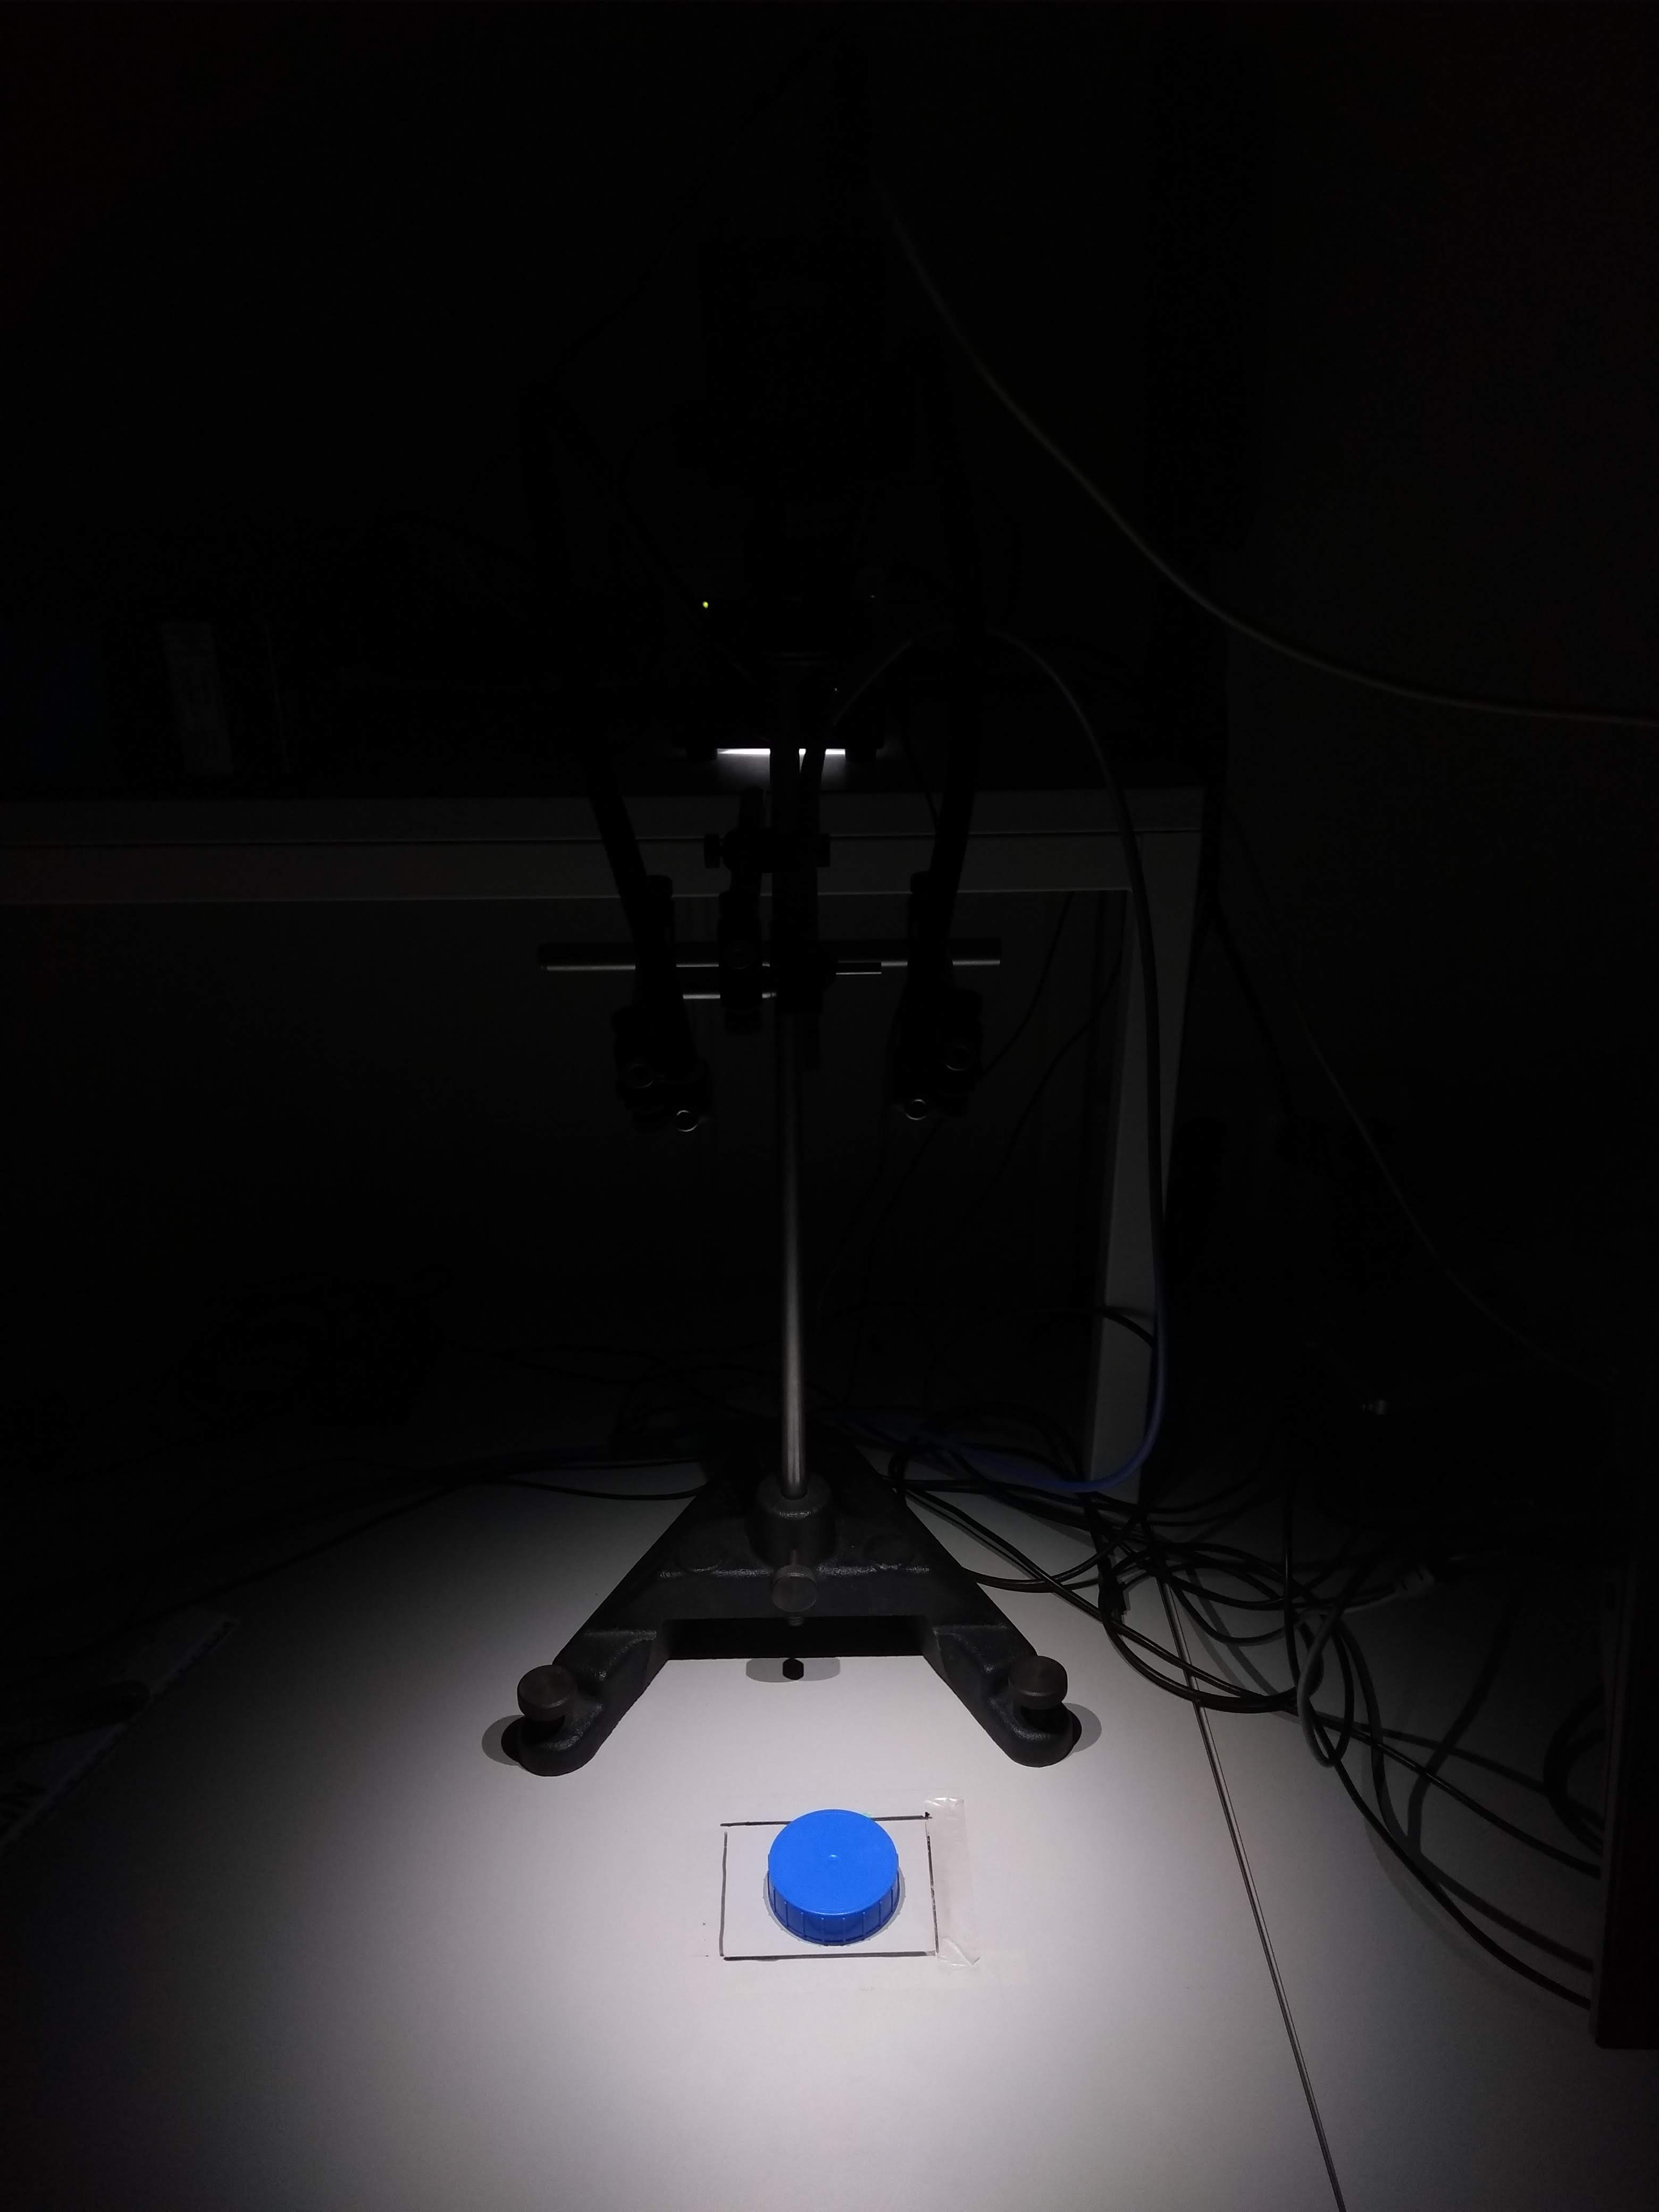
\includegraphics[width=1\textwidth]{figures/picture_taking_in_the_dark}
    \caption{Photo of the setup unlit}
    \label{fig:picture_of_setup_unlit}
\end{figure}


\subsection{Images}

\begin{figure}[h]
    \begin{subfigure}{0.5\textwidth}
        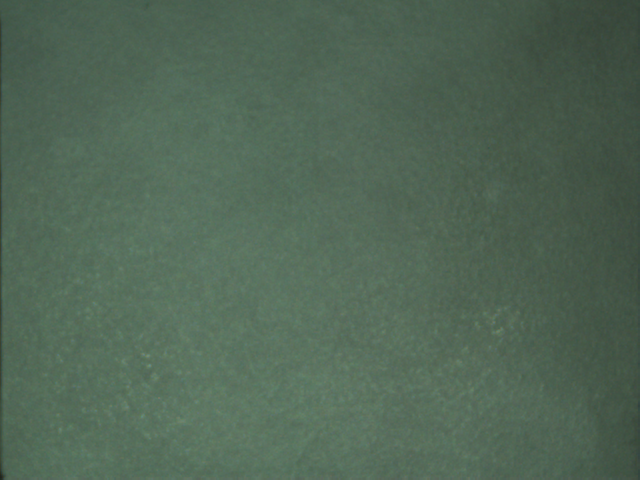
\includegraphics[width=0.9\linewidth, height=5cm]{figures/camera_pictures_png/001_background.png}
        \caption{001 Background, the reference picture}
        \label{fig:001_background}
        \end{subfigure}%
        \begin{subfigure}{0.5\textwidth}
        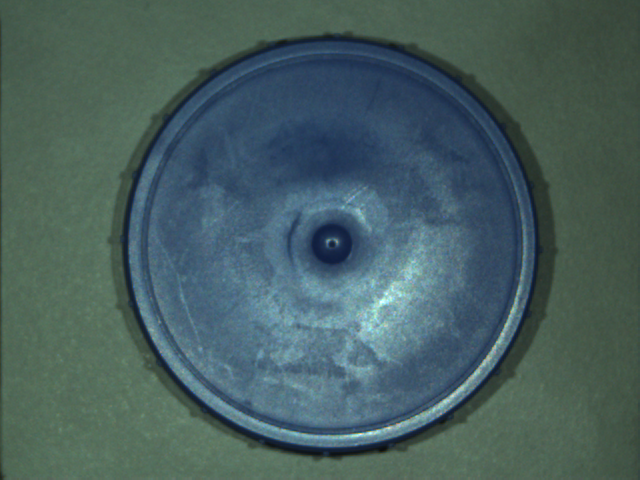
\includegraphics[width=0.9\linewidth, height=5cm]{figures/camera_pictures_png/002_blue_cap.png}
        \caption{002 Blue cap, the photo being analysed}
        \label{fig:002_blue_cap}
    \end{subfigure}
    
    \caption{Hadamard division}
    \label{fig:hadamard_division}
\end{figure}



\begin{figure}[h]
    \begin{subfigure}{0.5\textwidth}
        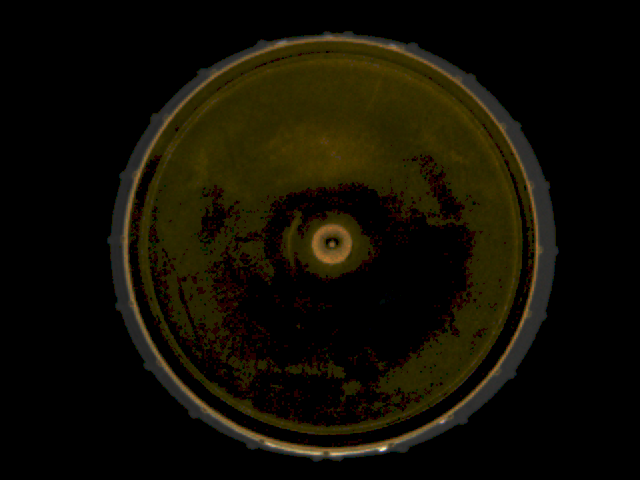
\includegraphics[width=0.9\linewidth, height=5cm]{figures/processed_camera_pictures/002_blue_cap_negative_difference.png} 
        \caption{The background divided by the with the blue cap}
        \label{fig:002_blue_cap_negative_difference}
        \end{subfigure}%
        \begin{subfigure}{0.5\textwidth}
        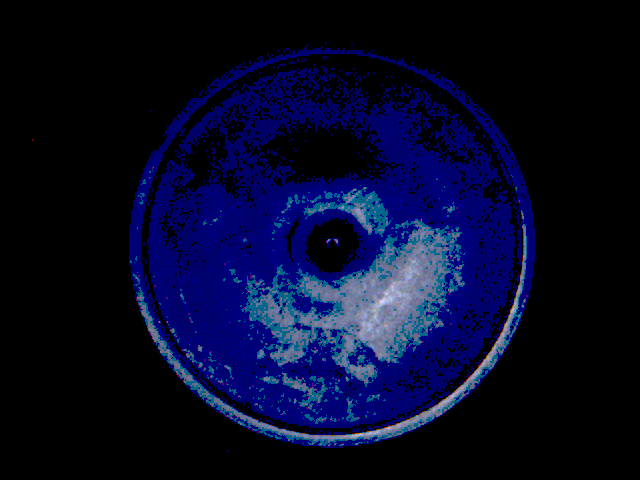
\includegraphics[width=0.9\linewidth, height=5cm]{figures/processed_camera_pictures/002_blue_cap_positive_difference.png}
        \caption{The image with the blue cap divided by the background}
        \label{fig:002_blue_cap_positive_difference}
    \end{subfigure}
    
    \caption{Hadamard division}
    \label{fig:hadamard_division}
\end{figure}


\subsection{Spectrum of camera}
Figure \ref{fig:relative_reflection_around_zero} shows nine plots, the first one shows the reference spectrum, the spectrum without any objects. The following eight plots shows the Relative Reflectance (\ref{eq:relative_reflectance}), their 

\begin{landscape}
\begin{figure}[t]
    \centering
    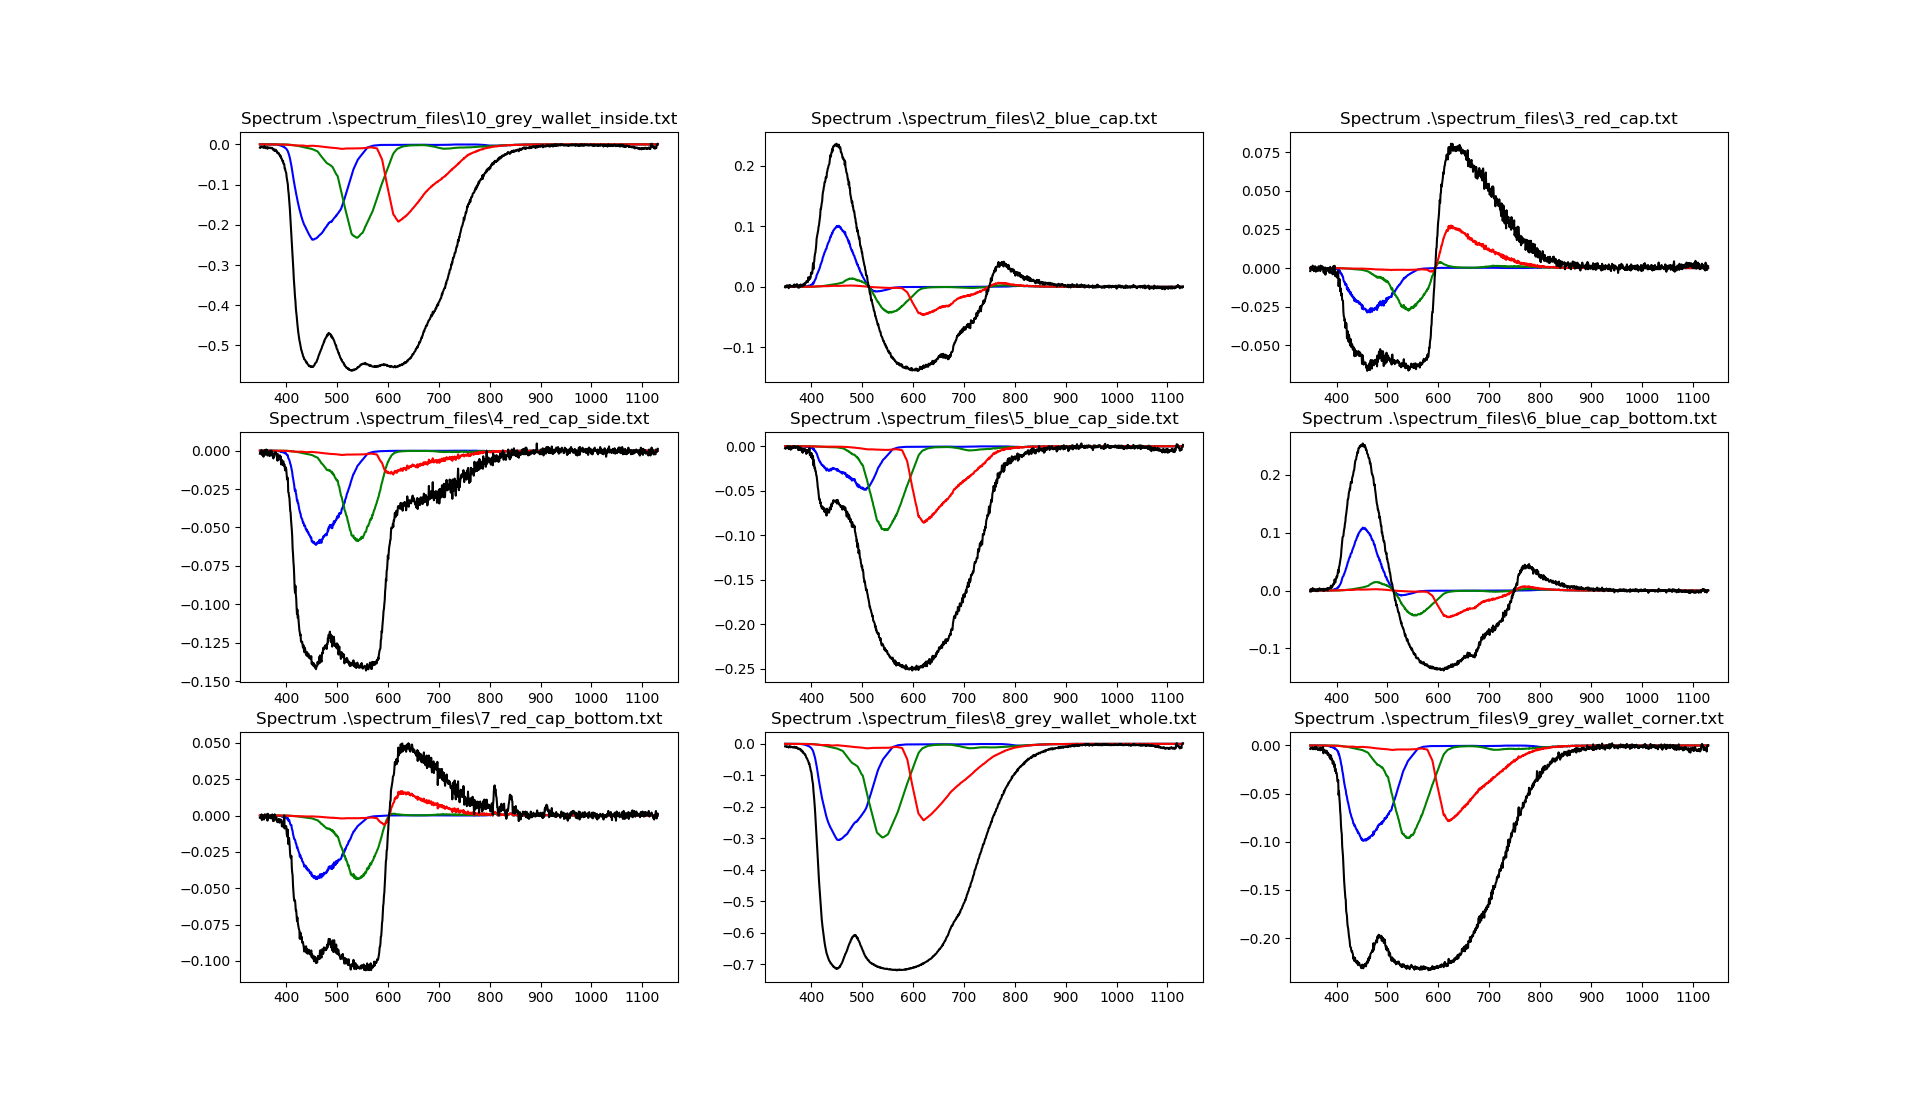
\includegraphics[width=1\paperwidth]{Plots/relative_reflectance_around_zero_with_qe_color_response.png}
    \caption{Relative reflection centered around zero}
    \label{fig:relative_reflection_around_zero}
\end{figure}
\end{landscape}


\subsection{Correlating Spectrometer to Camera}


\section{Conclusion}

It has proven very hard to correlate spectrometer and camera values that should be similar, even in ideal situations as in a dark lab.

\bibliographystyle{plain}
\bibliography{references.bib}
\end{document}